\chapter{Understanding phytoplankton community shifts in the eastern Cariaco basin}

\small {\textbf{This is the current state of progress towards the first manuscript}}


\normalsize
\section{Regime shift in the Cariaco Basin}
The CARIACO time-series has been collecting detailed data on the phytoplankton community in the Cariaco Basin from 1995 to 2017 (see Section \ref{CARIACOintro} for a full description). What has been a particular focus of the research based on this data set is the apparent changes in environmental conditions documented in both the physical boundary conditions as well as the biological data. 
As documented by \citet{Taylor2012}

and further investigated by \citet{Pinckney2015}

Interesting thing is that there was this shift in the PhytoplanktonCommunity but apparently no real reduction in Export! (This is in Taylor and Pinckney somehwere)
this would be coherent with Pinckney, no real reduction in biomass, but shifts in the community and towards greater depth, talk about depth of the euphotic zone! also have that data thanks to JP and CBN

\begin{figure}
\centering
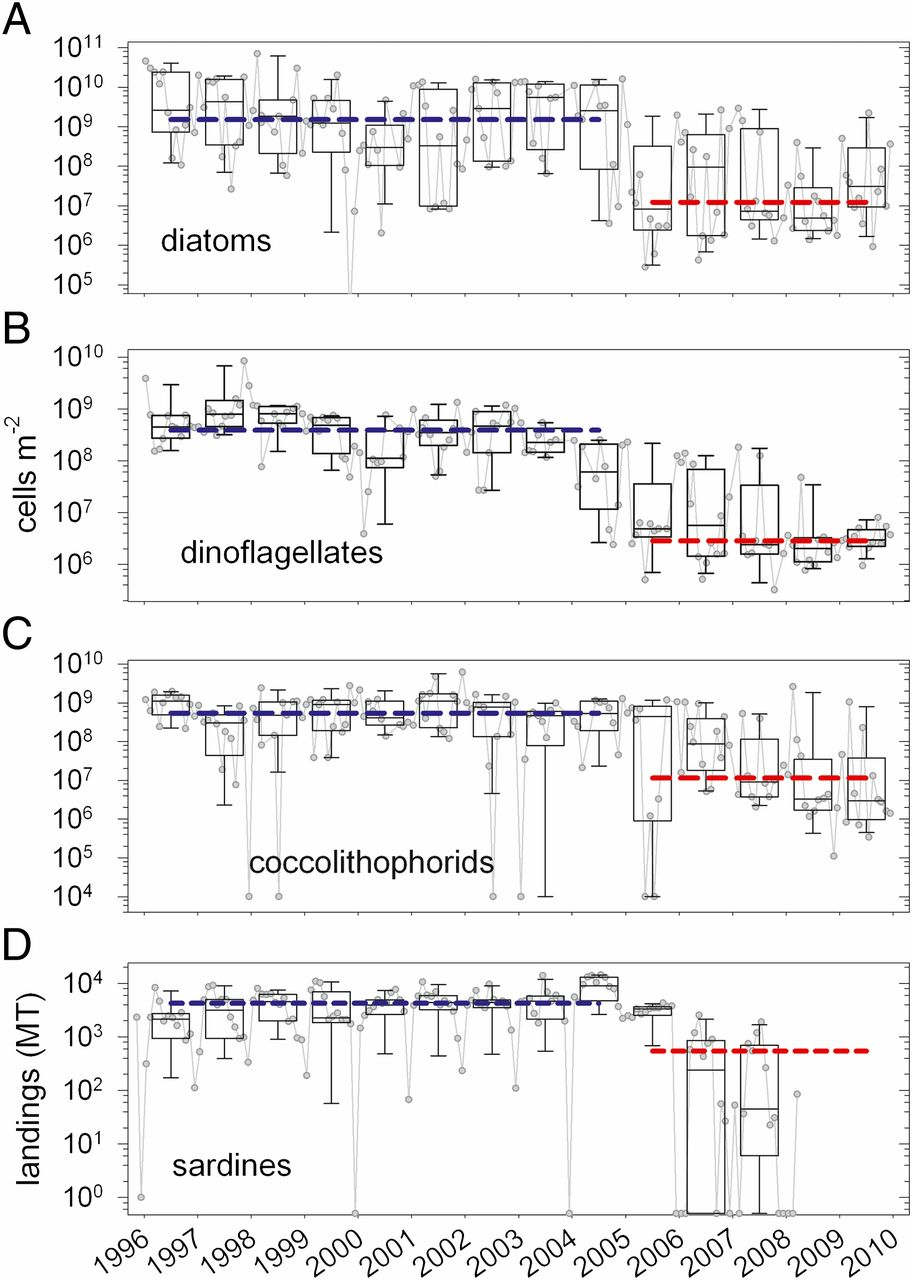
\includegraphics[trim = 0mm 0mm 0mm 0mm, clip, width=0.7\linewidth]{./Chp2-Pre/Tayloretal2012_F3.large.jpg}
\caption[Scheme]{\small {"Shifts in phytoplankton community composition and sardine landings from the southeastern Margarita Island fishery. Monthly observations presented as gray symbols. Box and whisker plots depict binned annual variations in diatom (A), dinoflagellate (B), coccolithophorid (C) inventories integrated over the upper 55 m and sardine fishery landings (D) in metric tons. Boxes represent the interquartile range of all observations (25th to 75th percentiles). Internal horizontal lines and whiskers are medians and 10th to 90th percentiles, respectively. Blue and red horizontal lines represent the grand medians of all observations between 1996 and 2004 and between 2005 and 2009, respectively. Data in early and late bins are significantly different in all cases (ANOVA; P < 0.001). [Fishery data are courtesy of L. W. Gonzáles (Universidad de Oriente, Boca de Río, Isla de Margarita, Venezuela); zero values artificially set at 0.5 for plotting purposes.)" from \citet{Taylor2012}}}
\label{TaylorSHIFTS}
\end{figure}




The term regime shift is actually not very well defined and has been used... \citep{DeYoung2004a}
There are global trends and indications of a regime shift, but methods to identify regime shifts are not well established and have been critically discussed in the literature \citep{Steele2004a, Mantua2004a, Litzow2016a}. To my knowledge no formal exploration of a potential regime shift has been performed with the CARIACO data, therefore the term regime shift is used here to describe the observed changes in the phytoplankton community and physical environment without presupposing a formally defined state shift in the entire ecosystem. 


\begin{figure}
\centering
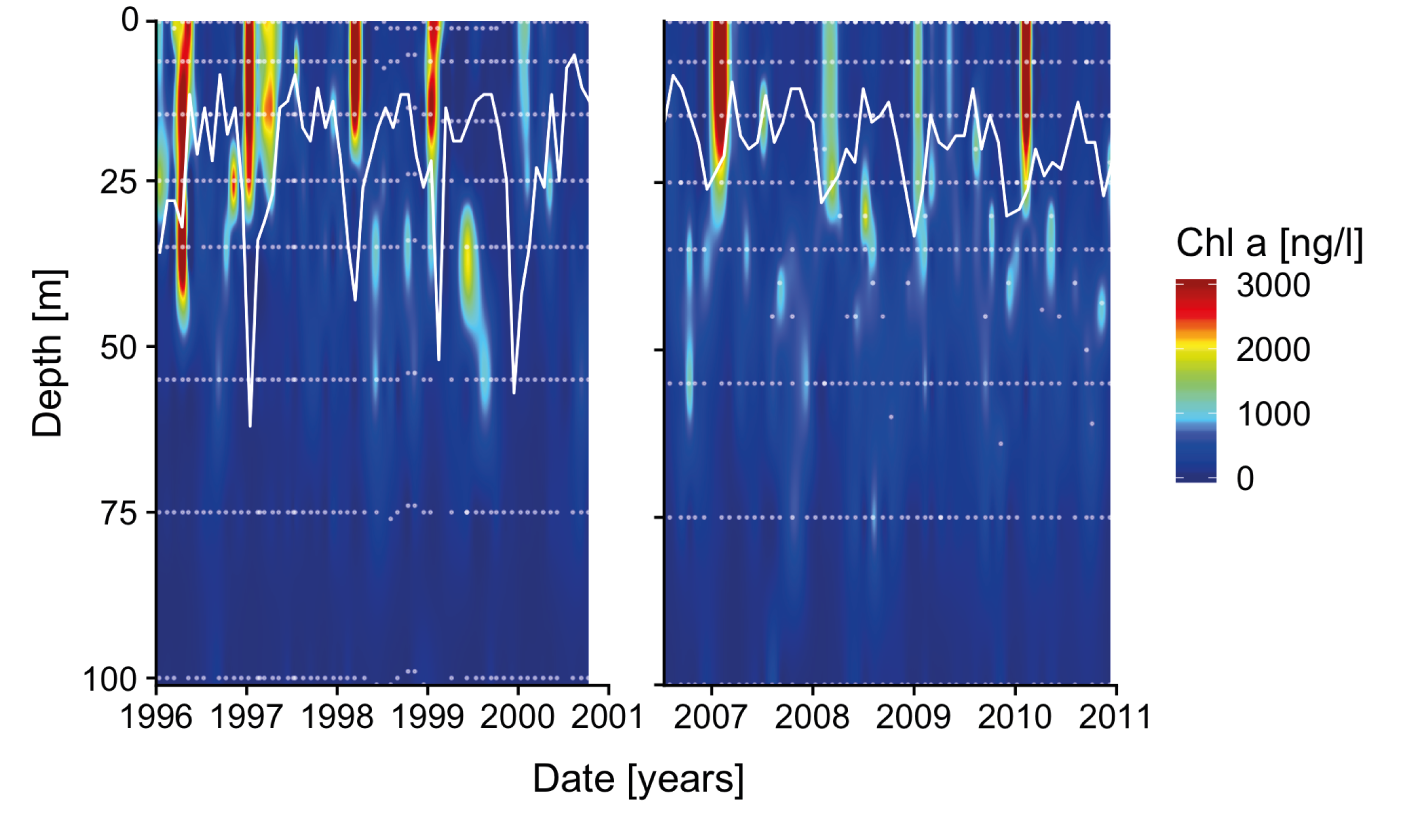
\includegraphics[trim = 0mm 0mm 0mm 0mm, clip, width=.9\linewidth]{./Chp2-Pre/Pinckneyetal2015_TotChlAcontoursMLD.png}
\caption[Scheme]{\small {Contour plot of HPLC-measured $chl~a$ for the two time periods with full data coverage (January 1996 to October 2000 and July 2006 to December 2010). Light white dots indicate data points. White line shows the depth of the mixed layer. HPLC Data and MLD depth was received from James Pinckney and Claudia Benitez-Nelson.}}
\label{TChlAPinckney}
\end{figure}


Talk about the data again

Also talk about mutshinda et al studies!
Mutshinda study one, bayesian approach: \cite{Mutshinda2013a}

Mutshinda study, same year, environmental factors: \cite{Mutshinda2013}

culminated in the study in PNAS: "Phytoplankton adapt to a changing environment" \cite{Irwin2015}

detailed phytoplankton data has been used in the previous studies for statistical analysis, but surprisingly not yet for ecosystem or trait-based modeling
This will be a first! first proper ecological model apart from this Export Flux model only including diatoms \citep{Walsh2002a}

FUNCTIONAL TYPES STRUCTURE --> explain linkage between Pigment Data that I use and functional diversity measurements (XMoreno et al. 2012X) take this from Pinckney et al. 2015...
Thus, photopigment-based measures offer an efficient way to quantify community or functional diversity (X Moreno et al., 2012 X). (From Pinckney et al 2015) ..> this would also be good to discuss in part 4!

bb


LOOKING AT BIOMASS DYNAMICS, leading over from Intro where i mentioned JP CBN data at the end (ad-lib)
XXX

\begin{figure}
\centering
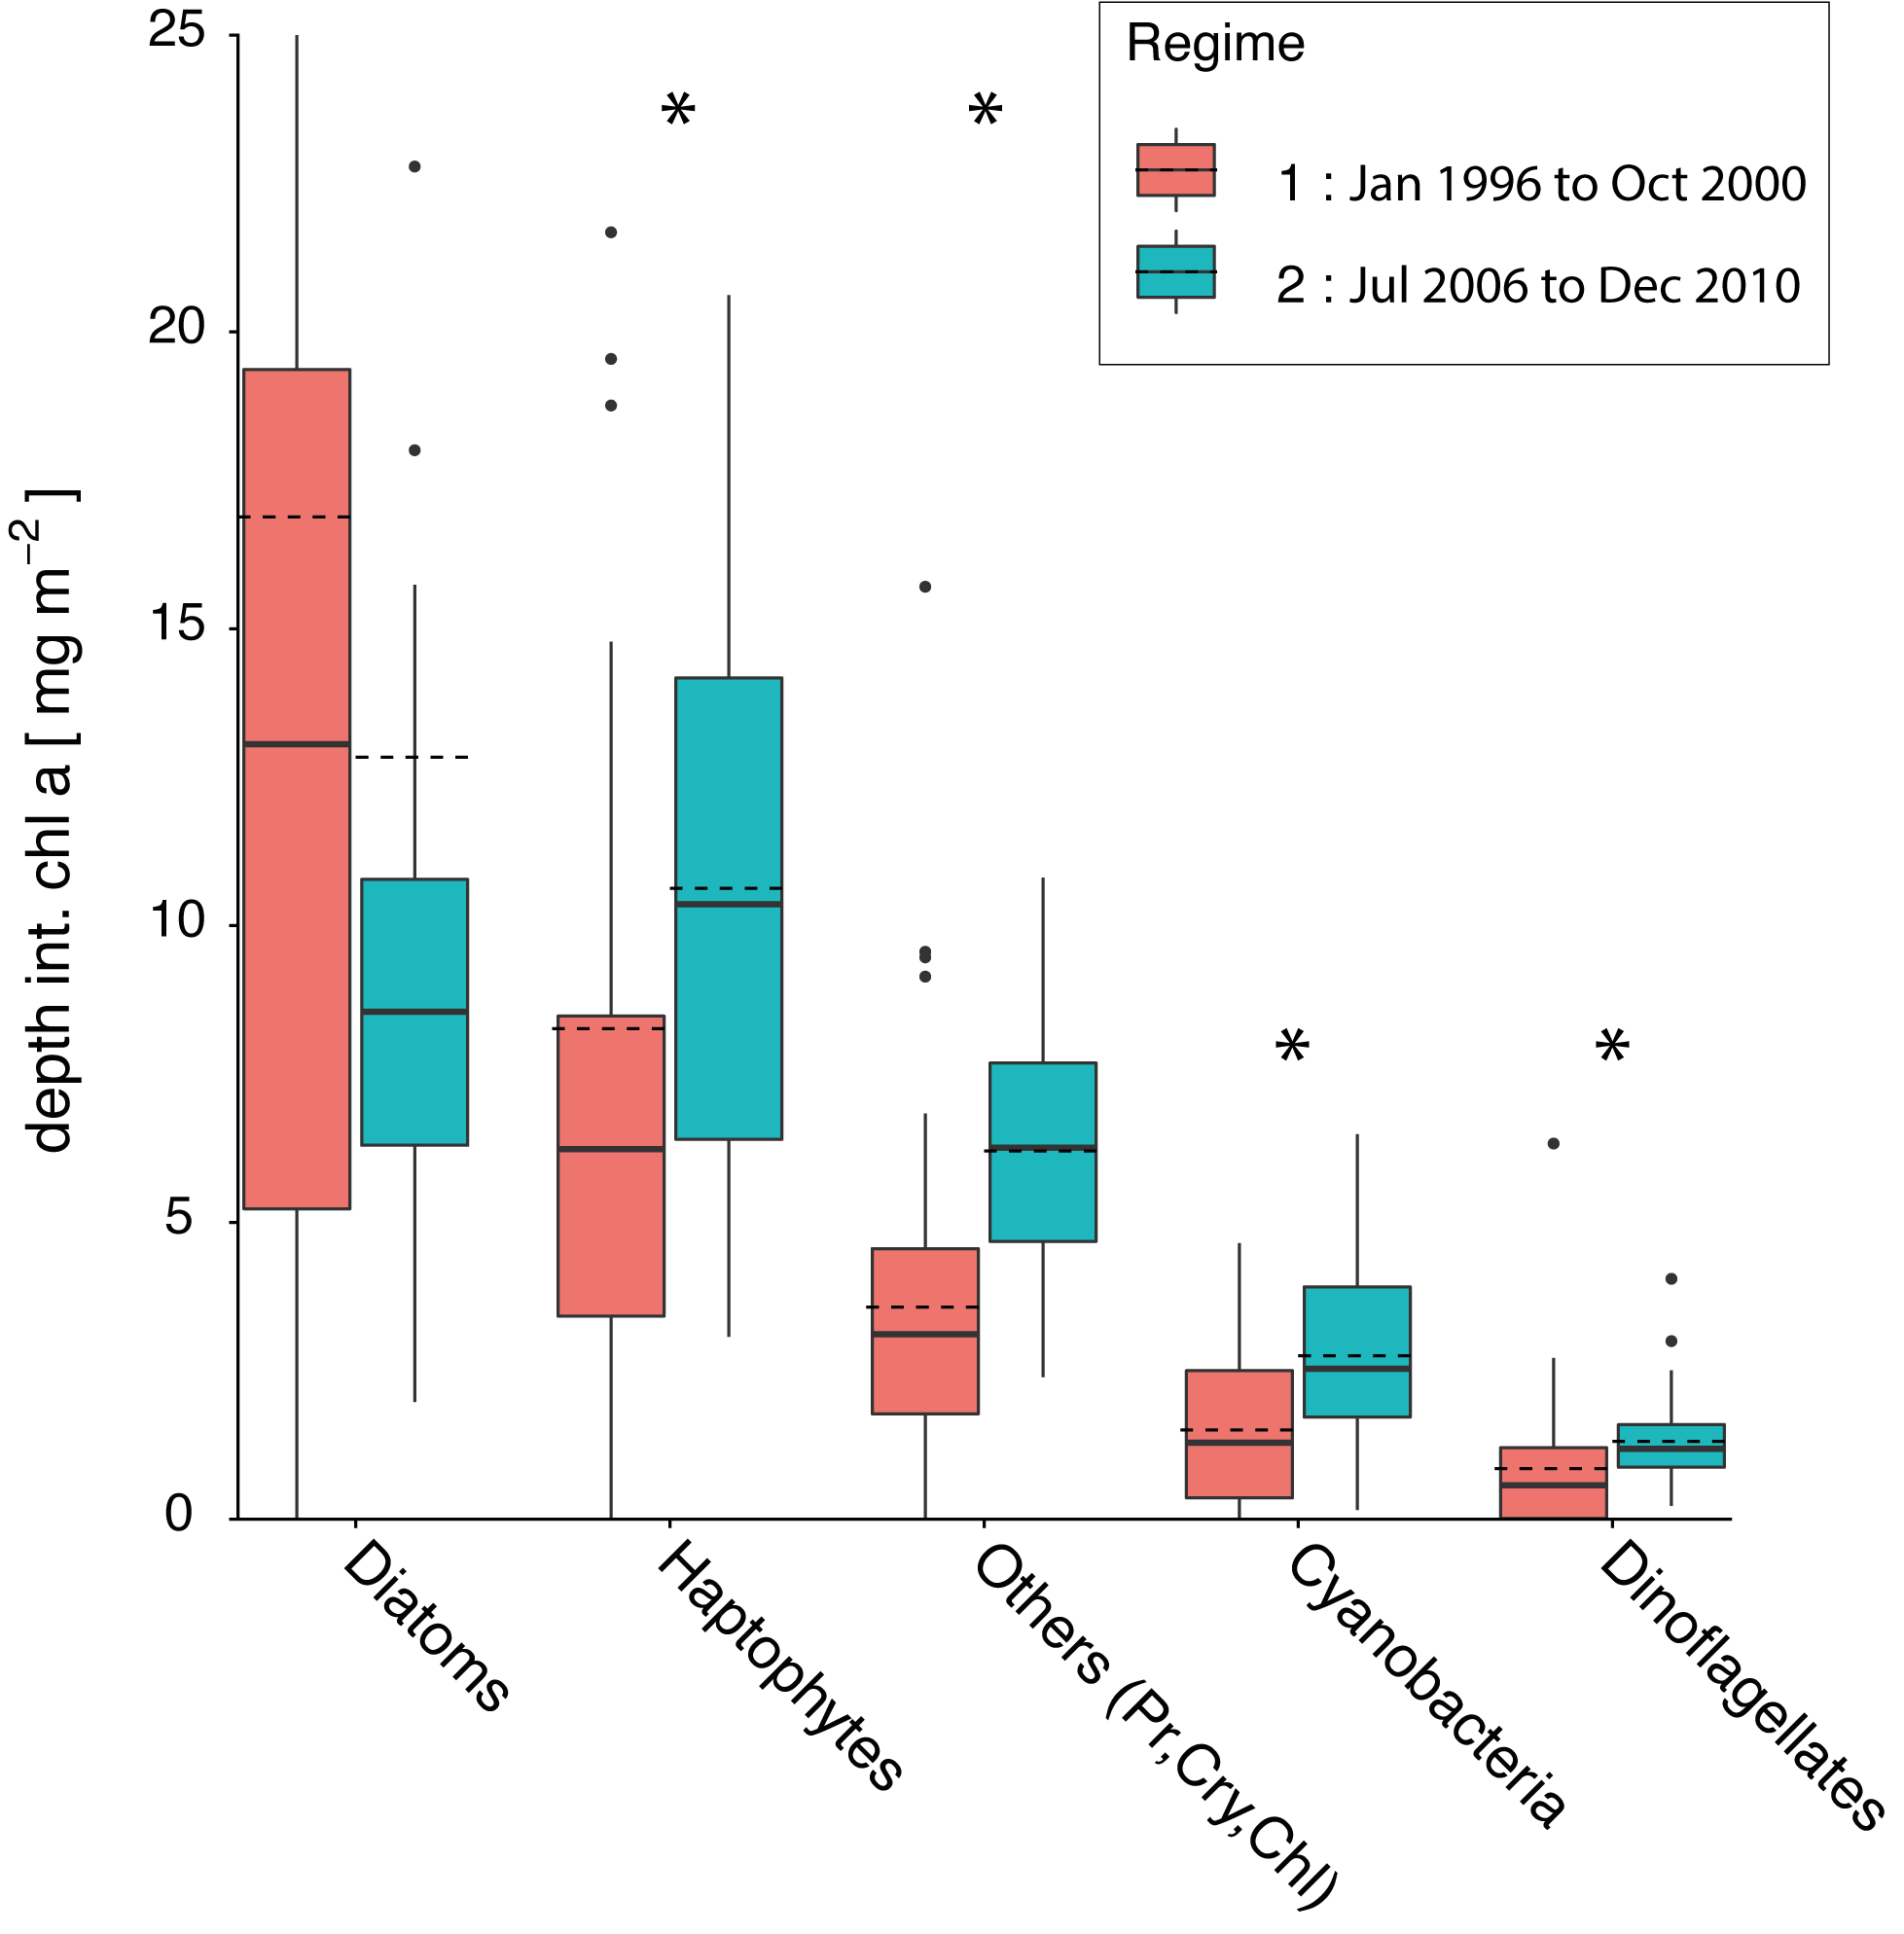
\includegraphics[trim = 0mm 0mm 0mm 0mm, clip, width=.7\linewidth]{./Chp2-Pre/PFT_groupsAsset511.png}
\caption[Scheme]{\small {Boxplots of HPLC-measured $chl~a$ depth integrated to 100 m for the two time periods with full data coverage. Boxplots illustrate the 25th and 75th quartiles (the box), the whiskers show the 5th and 95th percentiles, full line shows the median, dotted line shows the mean value per regime. Asterisk * indicates a significant difference between Times 1 and 2 in a one-sided t-test (p \textless	 0.05). Functional type $chl a$ was separated using the software Chemtax as described in \citet{Pinckney2015} The analyzed data was received from James Pinckney and Claudia Benitez-Nelson.}}
\label{PFTcariaco}
\end{figure}

EXPLAIN THE HYPOTHESES HERE; AND HOW THEY CAN BE TESteD

Main hypothesis, based on top down and bottom up processes:
Top down grazing has great influence on ecosystem, not just from biomass, but also biodiversity aspects \cite{Prowe2012c}.


\section{Methods}

MODEL STRUCTURE: 

- Cyanos as of yet not implemented as nitrogen fixers, given simplicity of model formulation, but actually are present and could be included: \citep{Montes2013}

dont really go into depth here, just generally state how things are done, python, odeint, system of ODEs

COPY METHODS SECTION FROM PhytoSFDM in a way, but with the current model setup
including the equations and allofthat!


\begin{figure}
\centering
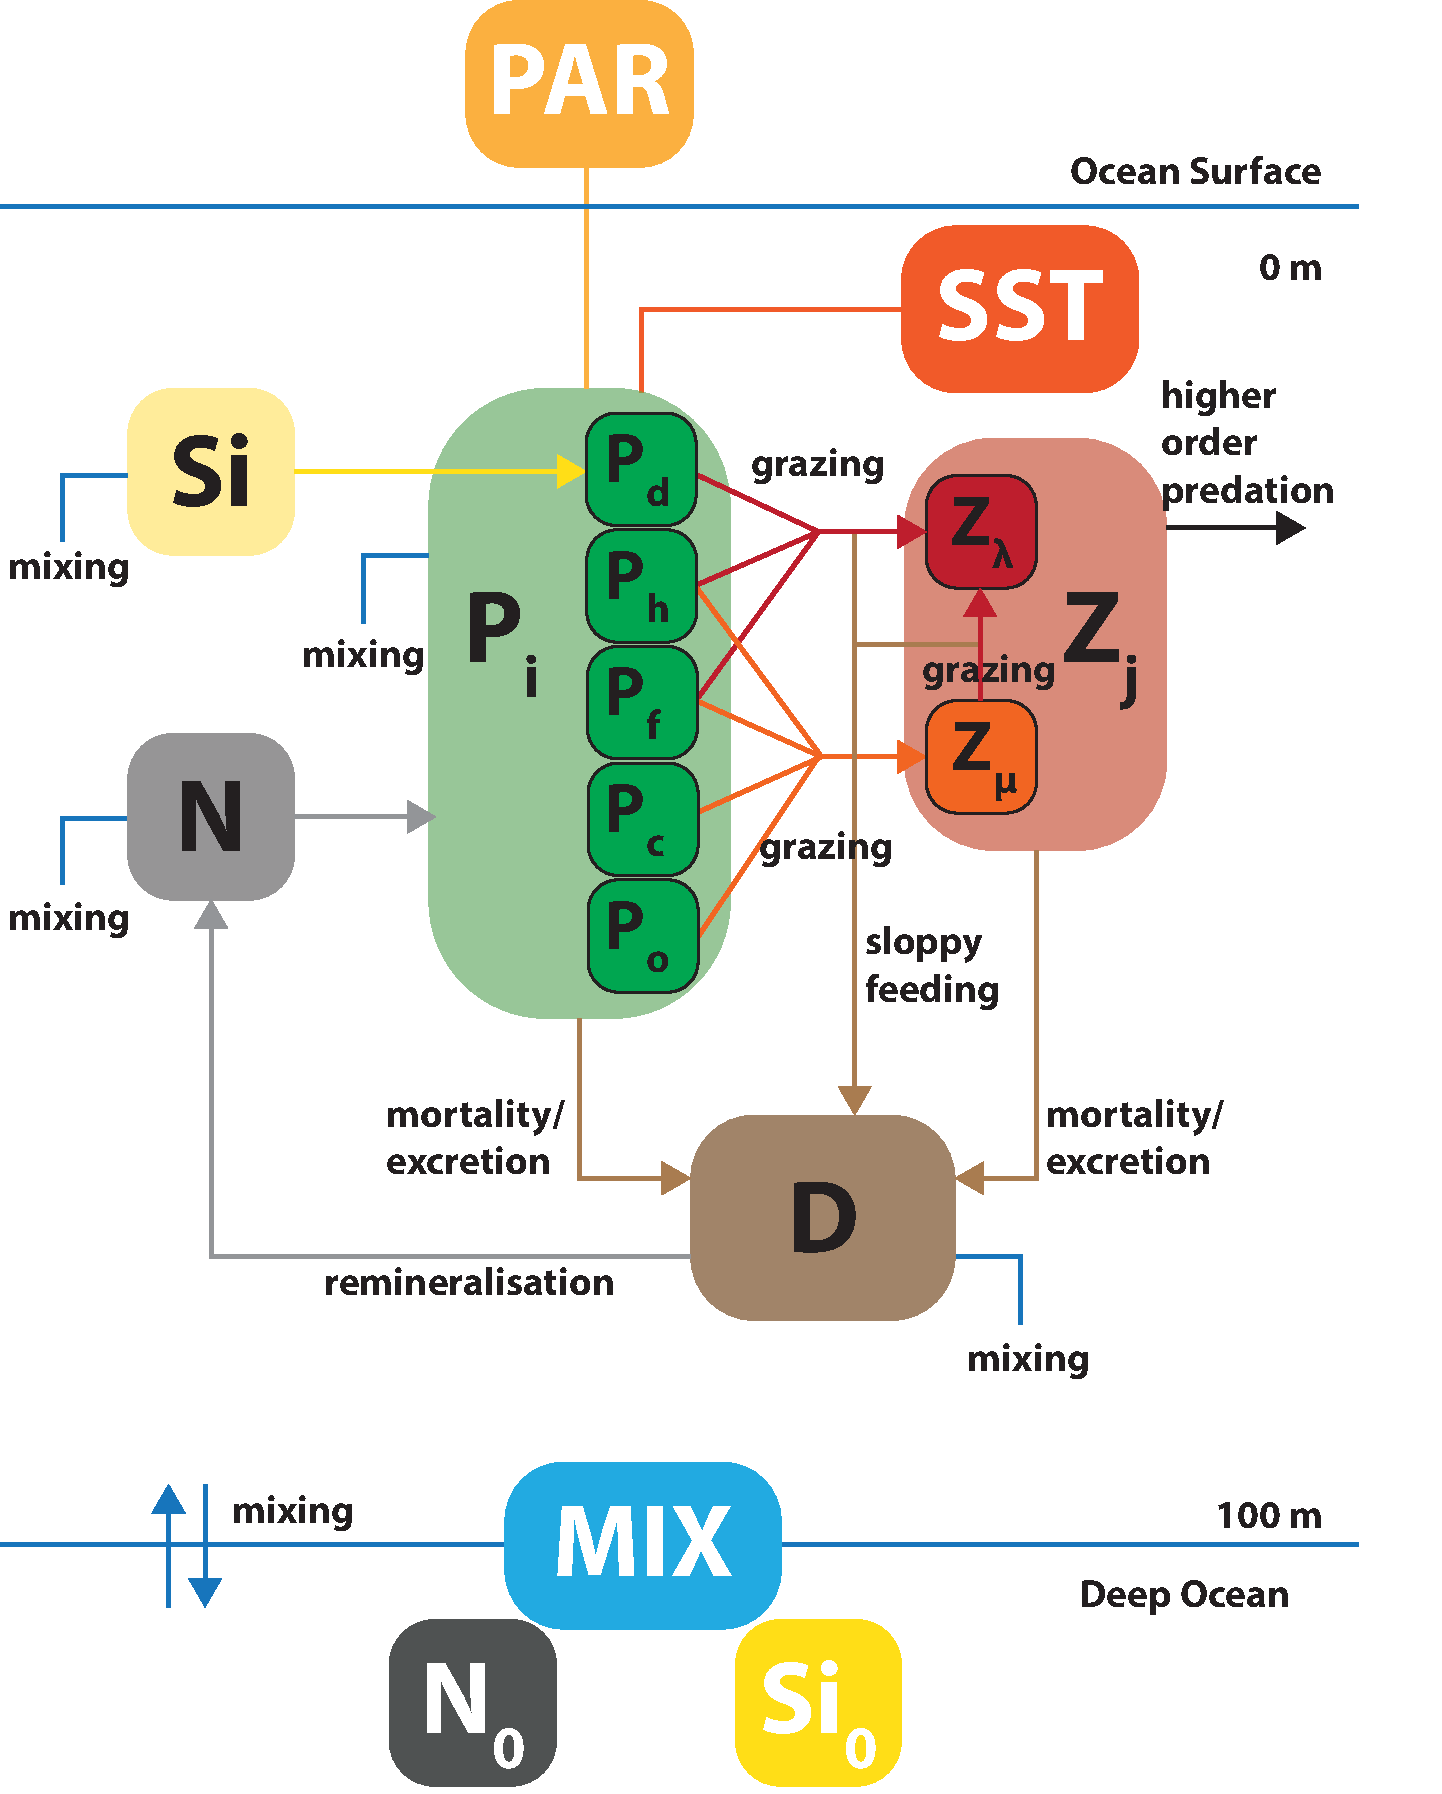
\includegraphics[trim = 0mm 0mm 0mm 0mm, clip, width=1.\linewidth]{./Chp2-Pre/ModelSchematicsAsset1111.pdf}
\caption[Scheme]{\small {Model schematics of current iteration of the ecosystem model.The ecosystem is embedded in a box of fixed depth. Nutrients below are assumed to be constant, mixing is a function MLD to simulate seasonal upwelling. XXXX}}
\label{ModelSchematics}
\end{figure}
XXXX

FORCING DATA

\begin{figure}
\centering
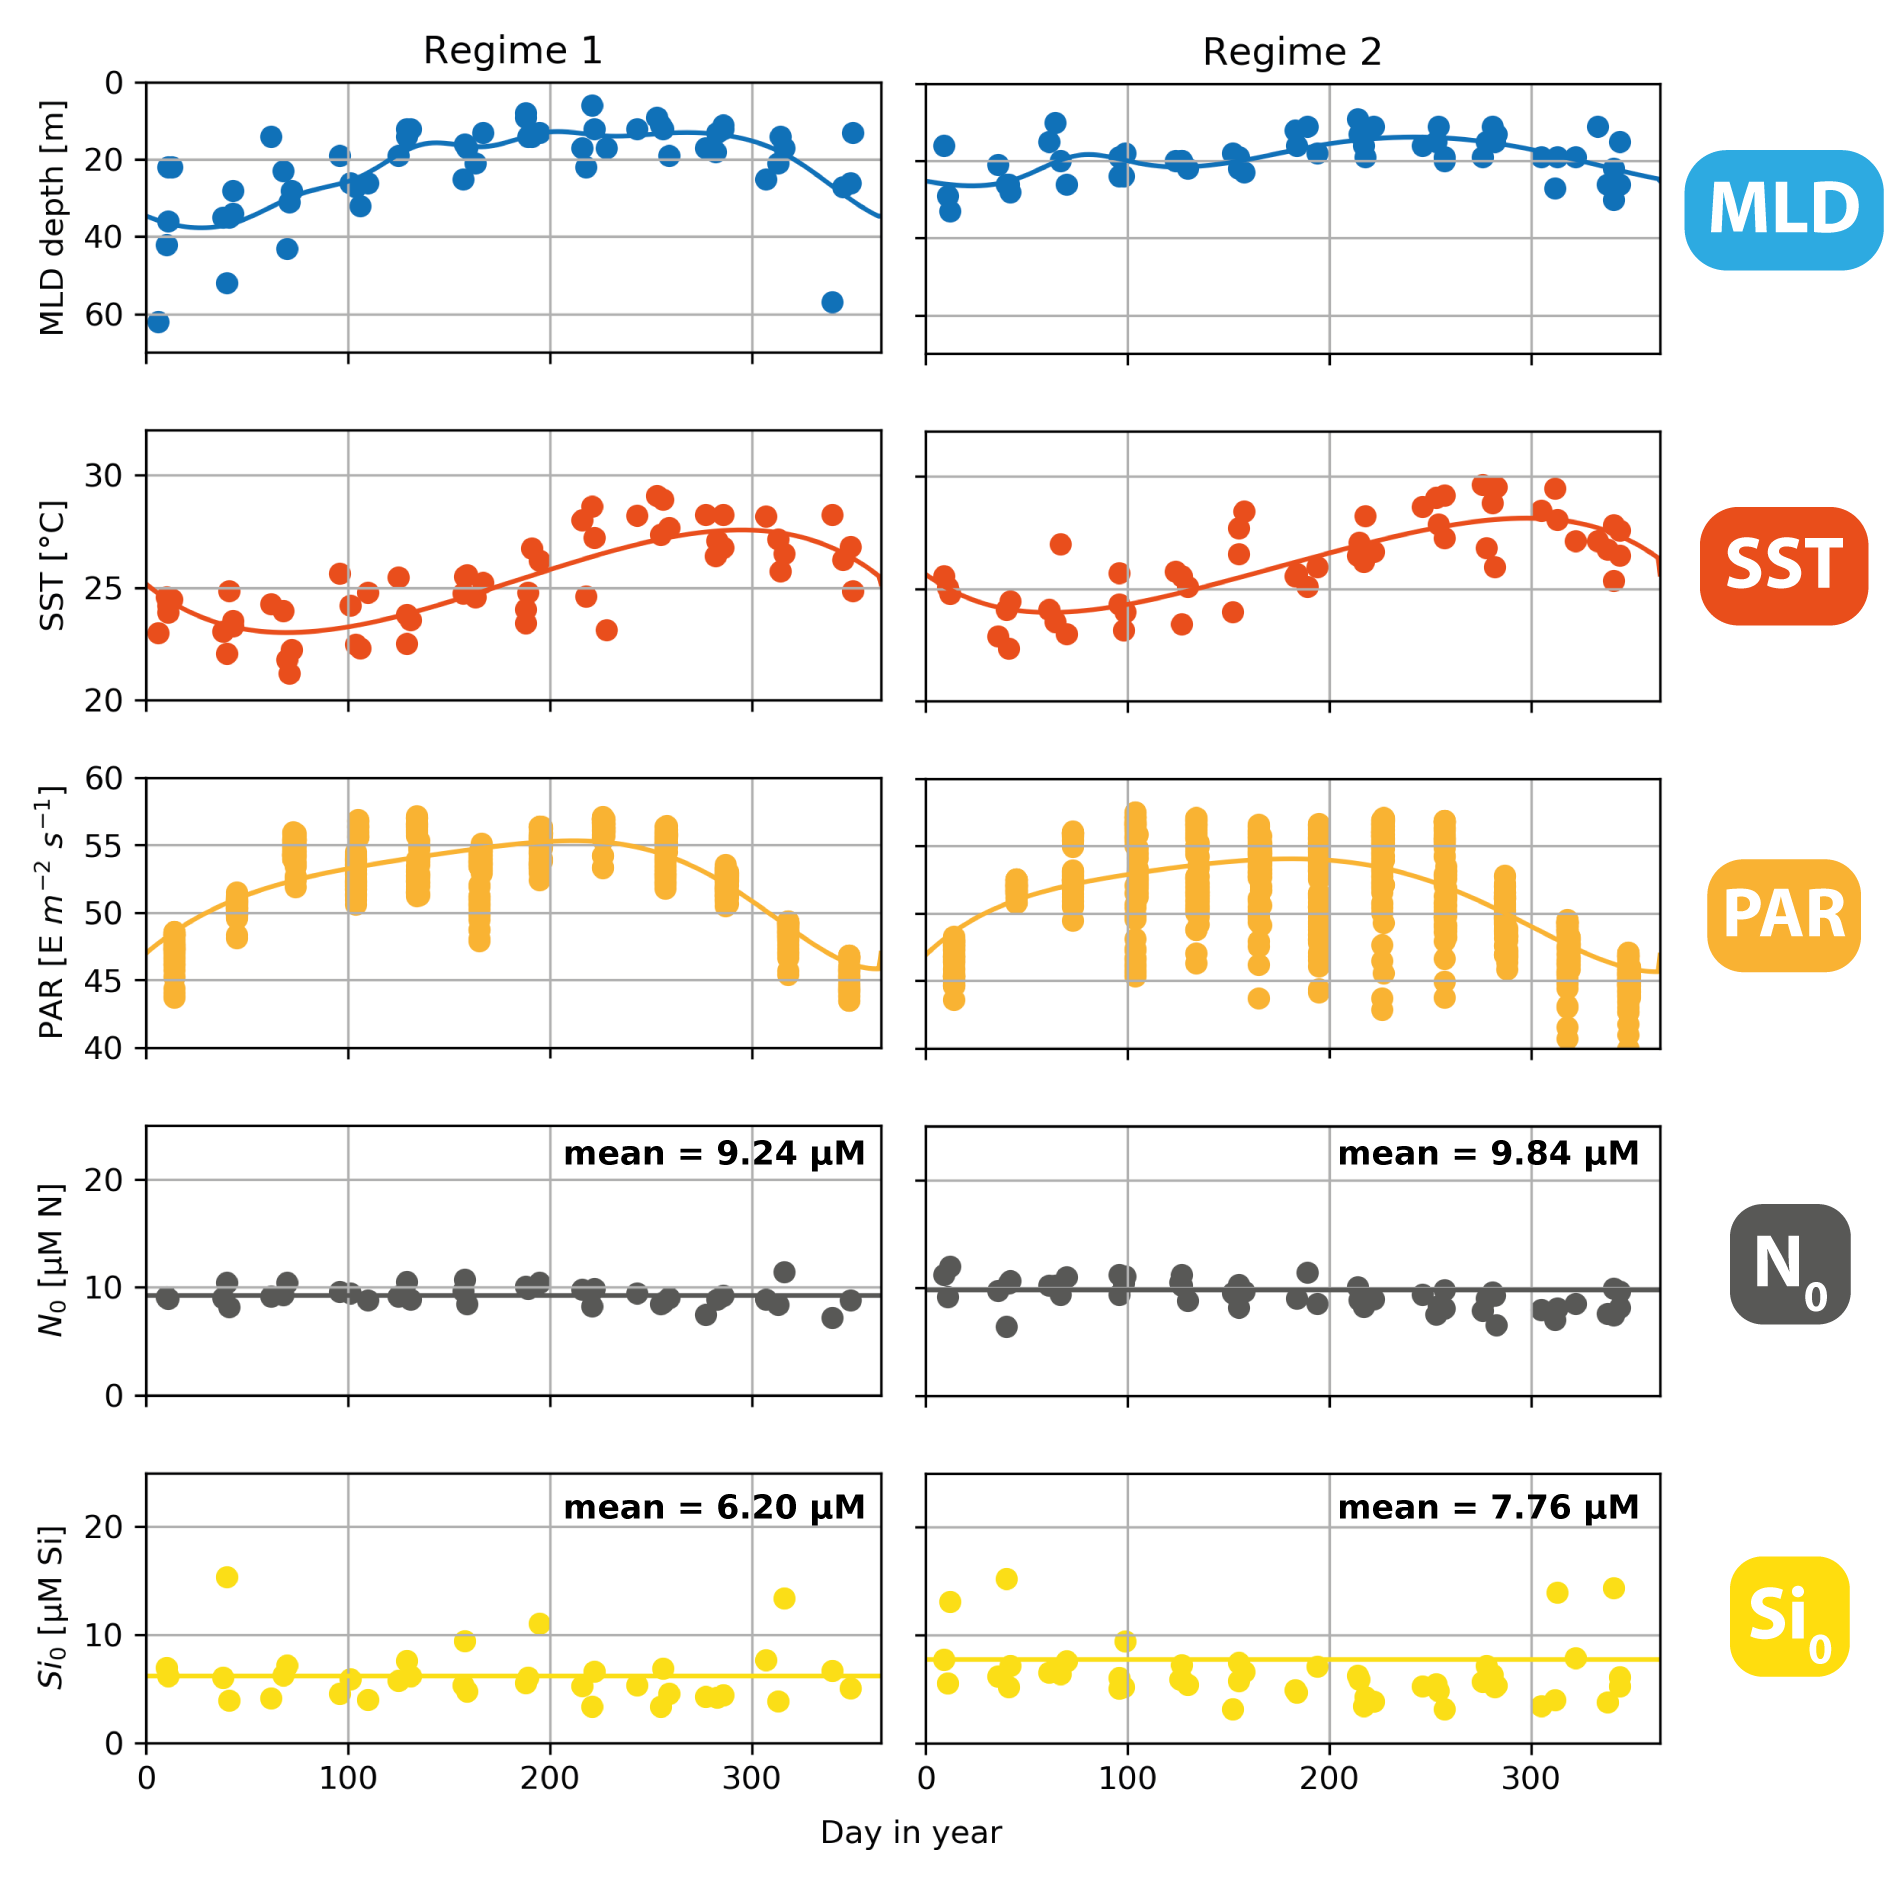
\includegraphics[trim = 0mm 0mm 0mm 0mm, clip, width=1.\linewidth]{./Chp2-Pre/ForcingAsset411.png}
\caption[Scheme]{\small {Aggregated forcing per the two regimes adapted from \citet{Pinckney2015}. Regime 1 from January 1996 to October 2000, Regime 2 from July 2006 to December 2010, values are aggregated to a single year. Depth profiles of Nitrate and Silicate were interpolated to depth and averaged between 100 and 150 m. Continous line shows interpolated values of MLD, PAR and SST used for model forcing and mean values for N and Si due to the assumption of a constant value at depth. SST and PAR data is taken from SeaWiFS satellite monthly climatological data. }}
\label{ModelForcing}
\end{figure}

\small {\textbf{Model physics in a tropical coastal setting}}

xXXX

Most models built for temperate oceans, since that is where reasearch (and funding) has been most well developed. Fasham NPZD type slabe physics explain.
Why won't this fit well in the Cariaco setting? - mostly due to shallow and comparatively invariable MLD, and nutrient fluxes don't correlate.
Problem of nutrient forcing! If MLD driven, nutrients below MLD are highly variable, only below 100m do we get towards a relatively constant N0 and Si0 (can show plots here!)


\begin{figure}
\centering
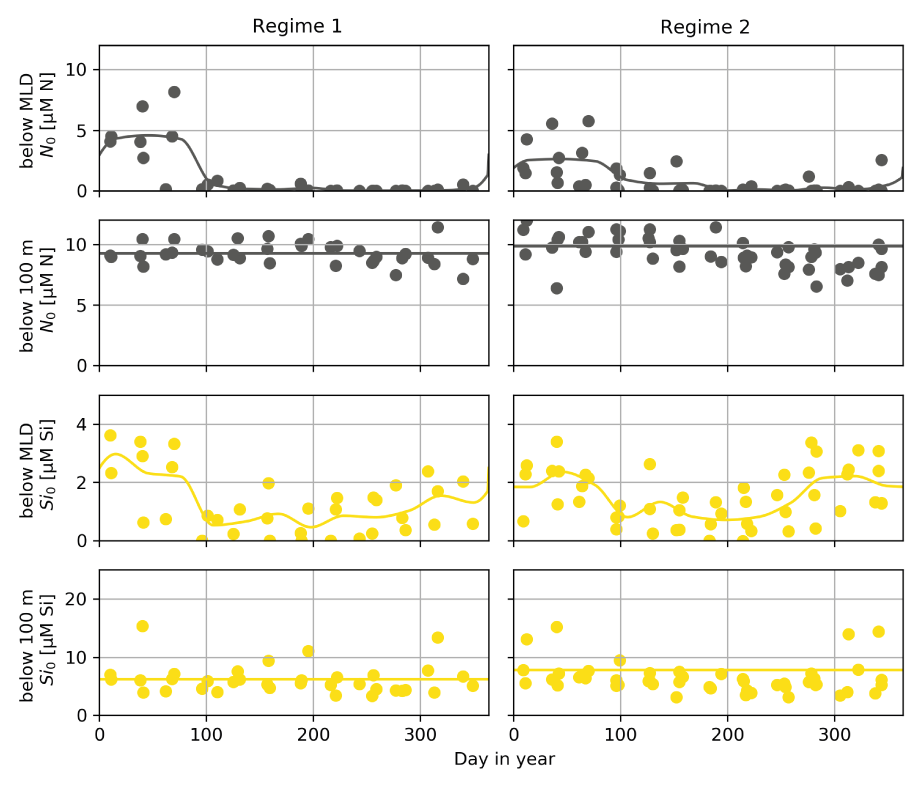
\includegraphics[trim = 0mm 0mm 0mm 0mm, clip, width=0.68\linewidth]{./Chp2-Pre/NutsBELOWmldAsset1011.png}
\caption[Scheme]{\small {Nutrient concentrations below MLD and averaged between 100 and 150 m depth for both regimes aggregated to one year. For values below MLD the continuous line represents interpolated forcing, for values below 100 m the line shows the mean value.}}
\label{BelowMLD}
\end{figure}

Moved from slab physics of PhytoSFDM model \citep{Acevedo-Trejos2016} which is based on Fasham \citep{Evans2003,Fasham1990a} to a box model formulation adapted from Tyrrell \citep{Tyrrell1999}
The specific differences are (show equations):

HERE I CAN SHOW THE DIFFERENT MODEL RUNS, explain the difference
for this box model needs to get running! This won't be so easy.. so plan ample time my friend!

XXXX

XXXX

XXX

{\bf {\large A1. CARIACO model description}} 

NPZD models are simplified marine ecosystem models that can be adapted to different physical settings and food web structures. For this model, the basic structure is inspired by the models of Fasham (1990) as it was adapted by Anderson et al. (2015). The pyhsical setting of the model uses a zero-dimensional slab structure as originally presented in Evans and Parslow (1985) and adapted from Acevedo-Trejos et al. (2015) where the ecosystem is described within a seasonally varying surface mixed layer above a deep homogenous layer. The code structure is the PhytoMFTM model written in the open source programming language Python, which provides a flexible framework for NPZD-type models with multiple functional types of phytoplankton and zooplankton. The model code and all statistical scripts are available publicly on Github (\url{https://github.com/ben1post/BennyPhD}).

The model framework was adapted to the setting of the CARIACO time-series in the Cariaco basin of the coast of Venezuela. The data includes phytoplankton species counts and two size-classes of zooplankton, which were included in the model as the 4 most prominent phytoplankton types, and 2 zooplankton types. The phytoplankton types include Nanoflagellates $P_{n}$, Diatoms $P_{dt}$, Coccolithophores, $P_{c}$ and Dinoflagellates $P_{dn}$. There are two Zooplankton types split by size class, named Mikrozooplankton $Z_{\mu}$ and Mesozooplankton $Z_{\lambda}$. 

Nitrogen $N$ (and Silicate $Si$ for Diatoms) is assimilated by the phytoplankton types $P_i$, which are grazed by the zooplankton types $Z_j$. Mortality of and excretion from phytoplankton and zooplankton, and sloppy feeding by zooplankton contribute to Detritus $D$. In addition to the linear mortality of $P_i$ and $Z_j$, there is an additional quadratic mortality term acting on $Z_j$, which represents higher-order predation on zooplankton.

{\bf {\large A1.1 Physical setting}}

The ecosystem component of the model is set within a zero-dimensional physical environment. The water column is divided into a 2-layer structure. A depth variable layer (e.g. the thermo- and/or pycnocline) separates a well-mixed surface layer containing the ecosystem component from a homogenous deep ocean. Concentrations of nutrients are averaged across the mixed layer, and remain constant below.  There is no lateral advection, but vertical mixing is modeled as a function of mixed layer depth (MLD) over time $M(t)$. Temperature depth profiles have been used to reconstruct the MLD at the investigated location. The derivative of MLD over time is given as $h(t) = dM(t)$. Exchange between the two layers is described by the two processes of turbulent diffusion and entrainment or detrainment caused by a shallowing or deepening of MLD. Adapted from Fasham (1993), the effects of entrainment and detrainment on nutrients, phytoplankton and detritus are given by the term $h^{+}(t)= max[h(t),0]$. Zooplankton is assumed to be able to maintain themselves within the mixed layer depth, therefore entrainment and detrainment of $Z_j$ are described by $h(t)$. Diffusive mixing between the layers has been parameterized with a constant factor $k$. The entire diffusion term is thus
\begin{equation}
\kappa = \frac{k + h^{+}(t)}{M(t)}
\end{equation}
In addition to the MLD interpolated from time series data, the model is externally forced with sea surface temperature (SST) taken from in situ data and interpolated from monthly to daily values and photosynthetically active radiation (PAR) from 8-day averaged SeaWIFs satellite data.

{\bf {\large A1.2 Phytoplankton}}

Phytoplankton growth is a function of light (PAR), temperature (SST) and nutrients. These factors are assumed to independently limit growth, so that (exemplary for $P_{d}$, i.e. diatoms) the growth term is
\begin{equation}
\mu_{d} = \mu_{d}^{max} \cdot U_{d}(N,Si)\cdot L_{d}(PAR)\cdot T_{d}(SST)
\end{equation}
where $\mu_{d}$ is the maximum growth rate per day and $T(PAR)$ is Eppleys formulation for temperature dependent growth (Eppley, 1972), given as $T(SST) = e^{0.063 * SST}$ with temperature in $^\circ C$. The light-limiting term $L(PAR)$ represents the integrated photosynthesis within the mixed layer as a function of incident irradiance at the surface $I_0$. Light attenuation is calculated using the Lambert-Beer law with irradiance at depth $z$ equal to
\begin{equation}
I(z) = I_0 \cdot e^{-k_{PAR} \cdot z}
\end{equation}
Here, $k_{PAR}$ is calculated as the sum of the constant attenuation coefficient of water $k_w$ and the self-shading of phytoplankton $k_c$ with the unit $\mu M^{-1}$ multiplied by total phytoplankton biomass $P$, i.e. $k_{PAR} = k_w + k_c P$. This model uses the Smith PI curve as a basis for the calculation, with $V_P$ representing the photosynthetic rate, $\alpha$, the initial slope of the PI curve and $V_p^{Max}$, the maximum photosynthetic rate
\begin{equation}
V_p = \frac{\alpha \cdot I \cdot V_p^{Max}} {\sqrt{(V_p^{Max})^2 + \alpha^2 \cdot I^2}}
\end{equation}
Combining equation (2) and (3) as presented in Anderson et al. (2015), the integrated photosynthesis $\bar{V}_p$ over depth $z$ is calculated as
\begin{equation}
\bar{V}_p(z) = \frac{V_p^{Max}}{k_{PAR} \cdot z} \cdot \ln \Bigg( \frac{\alpha \cdot I_0 + \sqrt{(V_p^{Max})^2+(\alpha \cdot I_0)^2}} {\alpha \cdot I(z) + \sqrt{(V_p^{Max})^2+(\alpha \cdot I(z))^2}} \Bigg)
\end{equation}
where $\bar{V}_p$ equals the light-limiting term $L$ in the growth equation (2).

Nutrient limited growth of the phytoplankton community is described via a Monod equation. 
\begin{equation}
U(N) = \frac{N} {k_N + N}
\end{equation}
For diatoms $P_d$ the nutrient limiting term depends on both nitrogen and silicate concentration within the upper layer. According to Liebig's law of the minimum, always the lower nutrient availability limits Diatom growth:
\begin{equation}
U_{d}(N,Si) = min \Big( \frac{N} {k_{d}^N + N}, \frac{Si} {k_{d}^{Si} + Si} \Big)
\end{equation}
All other phytoplankton types are nutrient-limited only by available Nitrogen as in equation (6). Phytoplankton mortality and excretion are parameterized as a linear constant rate $mo$. With $G_{\mu}$ as grazing by Microzooplankton and $G_{\lambda}$ as grazing by Mesozooplankton (defined below), the equations for all phytoplankton types $P_i$ can now be written as
\begin{equation}
\frac{dP_{i}}{dt} = \mu_{i} \cdot P_{i} - mo_{i} \cdot P - G_{\mu}(P_{i}) - G_{\lambda}(P_{i}) - \kappa \cdot P_{i}
\end{equation}

{\bf {\large A1.3 Zooplankton}}

Two zooplankton types are resolved in the model according to size-class, Microzooplankton $Z_{\mu}$ and Mesozooplankton $Z_{\lambda}$. Following Anderson et al. (2015) the grazing of, for example, $Z_{\lambda}$ on diatoms $P_d$ is formulated as follows

\begin{equation}
G_{\lambda}(P_{d}) = \Bigg( \frac{\mu^Z_{\lambda} \cdot \phi^{\lambda}_d \cdot P_d} 
							{(k^Z_{\lambda})^2 + \phi^{\lambda}_d \cdot P_d + \phi^{\lambda}_c \cdot P_c + \phi^{\lambda}_{df} \cdot P_{df} + \phi^{\lambda}_{n} \cdot P_{n} + \phi^{\lambda}_{\mu} \cdot Z_{\mu}} \Bigg) \cdot Z_{\lambda}
\end{equation}
$\phi^{\lambda}_{d}$ = $\rho^{\lambda}_{d} P_{d}$ , $\phi^{\lambda}_{c}$ = $\rho^{\lambda}_{c} P_{c}$ , $\phi^{\lambda}_{df}$ = $\rho^{\lambda}_{df} P_{df}$ , $\phi^{\lambda}_{n}$ = $\rho^{\lambda}_{n} P_{n}$ , $\phi^{\lambda}_{\mu}$ = $\rho^{\lambda}_{\mu} Z_{\mu}$

with $\mu^Z_{\lambda}$ as the maximum grazing rate, $k^Z_{\lambda}$ as the half saturation constant of grazing, $\phi^{\lambda}_{d}$ as the density dependent feeding preference of $Z_{\lambda}$ feeding on $P_d$, defined as $\rho_{d} \cdot P_{d}$, with $\rho^{\lambda}_{d}$ as the feeding preference coefficient.



{\bf {\large A1.x Solving method}}

The system of differential equations was solved numerically using the fourth-order Runge-Kutta method in the odeint function of the scipy package in python 3.7. 

Physical forcing is interpolated ... Taken from the regimes ... etc.


{\bf {\large Full System of equations}}

\begin{eqnarray}
\frac{\partial N}{\partial t} & = & 
\kappa \cdot \left(N_{0} - N\right) + 
\delta^{N}_{D} \cdot D -
\sum_{i=1}^{n_P} [\mu_i \cdot U_{i}(N_0,Si_0)\cdot L_i(PAR)\cdot T_i(SST) \cdot P_{i}] 
\nonumber \\
\frac{\partial Si}{\partial t} & = & 
\kappa \cdot \left(Si_{0} - Si\right) 
- \mu_{dt} \cdot U_{dt}(N_0,Si_0) \cdot L_{dt}(PAR)\cdot T_{dt}(SST) \cdot P_{dt}
\nonumber \\
\frac{\partial P_{i}}{\partial t} & = & 
\mu_{i} \cdot U_{i}(N_0,Si_0)\cdot L_{i}(PAR)\cdot T_{i}(SST) \cdot P_{i}
- m_{i} \cdot P_{i}
- \sum_{j=1}^{n_Z} [I^{tot}_j \frac{p^i_{j} \cdot P_{i}} {R_{j}} Z_{j}] -
\frac{v}{M(t)} \cdot P_{i} -
\kappa \cdot P_{i}
\nonumber \\
\frac{\partial Z_{\mu}}{\partial t} & = & 
\delta_Z \cdot I^{tot}_{\mu} \cdot Z_{\mu}-
\mu^{}_{\lambda} \frac{Z_{\mu}}{Z_{\mu}+k_{\lambda}} Z_{\lambda}-
\kappa_{Z} \cdot Z_{\mu} -
m_{\mu} \cdot Z_{\mu} - 
g_{\mu} \cdot Z_{\mu}^{2}
\nonumber \\
\frac{\partial Z_{\lambda}}{\partial t} & = & 
\delta_Z \cdot I^{tot}_{\lambda} \cdot Z_{\lambda}+
\delta_{\lambda} \cdot \mu^{}_{\lambda} \frac{Z_{\mu}}{Z_{\mu}+k_{\lambda}} Z_{\lambda}-
\kappa_{Z} \cdot Z_{\lambda} -
m_{\lambda} \cdot Z_{\lambda} - 
g_{\lambda} \cdot Z_{\lambda}^{2}
\nonumber \\
\frac{\partial D}{\partial t} & = & 
\sum_{j=1}^{n_Z} [(1-\delta_Z) I^{tot}_j \cdot Z_{j}] +
(1-\delta_{\lambda}) \cdot \mu^{}_{\lambda} \frac{Z_{\mu}}{Z_{\mu}+k_{\lambda}} Z_{\lambda}-
\sum_{j=1}^{n_Z} [m_j \cdot Z_{j}] +
\sum_{i=1}^{n_P} [m_i \cdot P_{i}] -
\kappa \cdot D -
\delta^{N}_{D} \cdot D
\nonumber
\end{eqnarray}
 
where:\\
\mbox{} \hspace{.5cm} $N_0=$ Nitrogen concentration right below mixed layer [$\mu M$],\\
\mbox{} \hspace{.5cm} $N=$ Nitrogen concentration above mixed layer [$\mu M$],\\
\mbox{} \hspace{.5cm} $v=$ sinking rate of $P_i$ [$m$ $day^{-1}$],\\
\mbox{} \hspace{.5cm} $M(t)=$ mixed layer depth at time point $t$ [$m$],\\
\mbox{} \hspace{.5cm} $\kappa = \frac{1}{M(t)} \cdot \left(h^{+}(t) + \kappa\right)$ Constant that parameterizes diffusive mixing across the thermocline, \\
\mbox{} \hspace{.5cm} $h^{+}(t) = \max\left(0, \frac{d}{d t} M(t)\right)$ Function that describes entrainment and detrainment of material,\\
\mbox{} \hspace{.5cm} $\delta^N_D=$ Remineralization rate of nitrogen component of detritus $D$ [$\mu M d^{-1}$],\\
\mbox{} \hspace{.5cm} $\mu_i=$Growth rate of phytoplankton type $i$ [$d^{-1}$],\\


\mbox{} \hspace{.5cm} $U_i=\begin{cases}\min\left(\frac{N}{N + U^{N}_i}, \frac{Si}{Si + U^{Si}_i}\right),& \text{if P-type is Diatom}\\\frac{N}{N + U^{N}_i}, & \text{otherwise}\end{cases}$ Nutrient uptake of phytoplankton $i$,\\

\mbox{} \hspace{.5cm} $L_i=\frac{1}{M(t) \cdot k_{w}} \cdot \left(e^{1 - \frac{PAR(t)}{Opt^{I}_i}} + e^{1 - \frac{PAR(t)}{Opt^{I}_i} \cdot e^{- M(t) \cdot k_{w}}}\right)$ Light dependence of  phytoplankton $i$,\\
\mbox{} \hspace{.5cm} $T_i= e^{0.063 \cdot SST}$ Temperature dependence of phytoplankton $i$,\\

\mbox{} \hspace{.5cm} $P_i=$ Biomass of phytoplankton type $i$ [$\mu M N$],\\
\mbox{} \hspace{.5cm} $m_i=$ Mortality/excretion rate for phytoplankton type $i$,\\

\mbox{} \hspace{.5cm} $I^{tot}_j= \mu^{Z}_j \cdot \frac{R_{j}}{R_{j} + k^Z_j}$ Total intake of zooplankton type $j$,\\
\mbox{} \hspace{.5cm} $k^Z_j =$ Half saturation constant of zooplankton type $j$,\\
\mbox{} \hspace{.5cm} $R_{j}= \sum_{i} (p_{i j} \cdot P_{i})$ Total ressource density of zooplankton type $j$,\\
\mbox{} \hspace{.5cm} $p^i_{j}=$ Feeding preference of zooplankton type $j$ feeding on phytoplankton type $i$,\\
\mbox{} \hspace{.5cm} $R_{\mu}= p^n_{\mu} \cdot P_{n} + p^{dn}_{\mu} \cdot P_{dn} + p^c_{\mu} \cdot P_{c}$ Total ressource density of Mikrozooplankton $Z_{\mu}$,\\
\mbox{} \hspace{.5cm} $R_{\lambda}= p^{dt}_{\lambda} \cdot P_{dt} + p^{dn}_{\lambda} \cdot P_{dn} + p^c_{\lambda} \cdot P_{c}$ Total ressource density of Mesozooplankton $Z_{\lambda}$,\\



\mbox{} \hspace{.5cm} $Z_j=$ Biomass of zooplankton type $j$ [$\mu M N$],\\
\mbox{} \hspace{.5cm} $\delta_{Z}=$ Grazing efficiency of zooplankton on phytoplankton (represents sloppy feeding), \\
\mbox{} \hspace{.5cm} $K_{Z}=\frac{1}{M(t)} \cdot \frac{d}{d t} M(t)$ Mixing term of zooplankton, \\
\mbox{} \hspace{.5cm} $g_{i}=$ Higher order predation on zooplankton (quadratic), \\
\mbox{} \hspace{.5cm} $m_{j}=$ Mortality/excretion rate for zooplankton type $j$,\\



\vspace{.2cm}
%
%{\it {\bf A1.1. Physical structure:}}\\
%
%It is a slab model for now, but might make sense to include depth layering, or euphotic zone depth, etc.. can take some of the cues for slab models from EMPOWER-1.0
%\vspace{.2cm}
%
%

\thispagestyle{empty}

\section*{PhytoMFTM model parameters (preliminary)}

\noindent
\begin{tabular}{llllllllll}

  symbol               & variable   & description & units   & value      & source\\
  \hline
  \multicolumn{3}{l}{Physical parameters:}\\
  \hline
  $\kappa$ & kappa & diffusive mixing constant & [$m$ $day^{-1}$] & 0.1/0.01 & [Fasham, 1990/1993]\\
  $\delta^{N}_{D}$ & deltaD\_N  & remineralization rate & [$day^{-1}$] & 0.05 & [Fasham, 1990]\\
  $k_w$ & kw & light attenuation coefficient & [$m^{-1}$] & 0.2 & [Edwards \& Brindley 1996]\\                           
  \multicolumn{3}{l}{affecting phytoplankton:} \\
  $v$ & v &  phytoplankton sinking constant & $[m day^{-1}]$ & 0.04 & [Edwards \& Brindley 1996]\\                      
  $I_{opt}$ & OptI & optimum irradiance & [$E$ $m^{-2}$ $day^{-1}$] & 30 & [Acevedo-Trejos, 2015]\\
  \\
  \hline
  \multicolumn{3}{l}{Phytoplankton parameters:}\\
  \hline
  $mo_P$ & moP &  mortality/excretion constant & [$day^{-1}$] & 0.09 & [Fasham, 1990]\\
  \\
  \multicolumn{3}{l}{functional type specific:} \\
  $P_{dt}$ & pt1  & Diatoms\\
  \hline
  $\Delta^{dt}_{Si}$ & pt1\_ratioSi & nitrogen to silicate ratio & [$\mu M Si$ $\mu M N^{-1}$] & 1.12 & [Brzezinski, 1985]  \\
  $K^{dt}_{Si}$ & pt1\_K\_Si & half-saturation constant of Si uptake & [$\mu M Si$] & 2 & [Kristiansen et al. 2000]\\
  $U^{dt}_N$ & pt1\_U\_N & half-saturation constant of N uptake & [$\mu M N$] &  0.446 & [Litchman et al. 2007]\\
  $\mu^{dt}_P$ & pt1\_muP & growth rate & [$day^{-1}$] & 1.5 & [Litchman et al. 2007]\\
  \\
  $P_{c}$ & pt2 & Coccolithophores\\
  \hline
  $U^{c}_N$ & pt2\_U\_N & half-saturation constant of N uptake & [$\mu M N$]  &  0.265 & [Litchman et al. 2007]\\
  $\mu^{c}_P$ & pt2\_muP  & growth rate & [$day^{-1}$]& 1.1 & [Litchman et al. 2007] \\
  \\
  $P_{dn}$ & pt3 & Dinoflagellates\\
  \hline
  $U^{c}_N$ & pt3\_U\_N & half-saturation constant of N uptake & [$\mu M N$]  &  0.009 & [Litchman et al. 2007]\\
  $\mu^{c}_P$ & pt3\_muP  & growth rate & [$day^{-1}$] & 0.6 & [Litchman et al. 2007]\\
  \\
  $P_{n}$ & pt4 & Nanoflagellates\\
  \hline
  $U^{n}_N$ & pt4\_U\_N & half-saturation constant of N uptake & [$\mu M N$]  &  0.045 & [Litchman et al. 2007]\\
  $\mu^{n}_P$ & pt4\_muP  & growth rate & [$day^{-1}$] & 1.7 & [Litchman et al. 2007]\\

  \\
  \hline
  \multicolumn{3}{l}{Zooplankton parameters:} \\
  \hline
  $mo_Z$ & moZ &  mortality/excretion constant & [$day^{-1}$] & 0.0125 & [Prowe et al. 2012]\\
  $\delta_Z$ & deltaZ & assimilation coefficient of grazing on $P_i$ & [-] & 0.75 & [Fasham, 1990]\\
  $\delta_{\lambda}$ & deltaLambda & assimilation coefficient of $Z_{\lambda}$ grazing on $Z_{\mu}$ & [-] & 0.75 & [Fasham, 1990]\\ 
  $\mu_{\lambda}$ & muIntGraze & maximum rate of $Z_{\lambda}$ grazing on $Z_{\mu}$ & [$day^{-1}$] & 0.05 & [?]\\
  $k_{\lambda}$ & kIntGraze & half-saturation constant of $Z_{\lambda}$ grazing on $Z_{\mu}$ & [$\mu M N$] & 0.5 & [?]\\ 
  \\
  $Z_{\mu}$ & zt1 & Mikrozooplankton\\
  \hline
  $\mu^{\mu}_Z$ & zt1\_muZ & maximum rate of grazing on $P_i$ & [$day^{-1}$] & 0.1 & [Prowe et al. 2012]\\ 
  $k^{\mu}_P$ & zt1\_Kp  & half-saturation constant of grazing on $P_i$ & [$\mu M N$] & 0.5 & [Prowe et al. 2012]\\
  $g_{\mu}$ & zt1\_pred & higher order predation on $Z_{\mu}$ & [$day^{-1}$] & 0.01 & [?]\\  
  \\
  $Z_{\lambda}$ & zt2 & Mesozooplankton\\
  \hline
  $\mu^{\lambda}_Z$ & zt2\_muZ & maximum rate of grazing on $P_i$ & [$day^{-1}$] & 0.1 & [Prowe et al. 2012]\\ 
  $k^{\lambda}_P$ & zt2\_Kp  & half-saturation constant of grazing on $P_i$ & [$\mu M N$] & 0.5 & [Prowe et al. 2012]\\
  $g_{\lambda}$ & zt2\_pred & higher order predation on $Z_{\lambda}$ & [$day^{-1}$] & 0.01 & [?]\\
  \\
  
  \hline
  \hline
\end{tabular}
\\\\\\\\
Feeding preferences: \\
\noindent
\begin{tabular}{l|l|l|l|l}
 
  & $P_{dt}$ & $P_{c}$ & $P_{dn}$ & $P_{n}$\\
\hline
$Z_{\mu}$ & 0 & 1 & 1 & 1\\
\hline
$Z_{\lambda}$ & 1 & 1 & 1 & 0\\
\hline
\end{tabular}
\\
where number is $p^i_j$ denoting feeding preference of $Z_j$ grazing on $P_i$



End Methods here

\section{Preliminary Results}


SHOW PROPER RUN, With Biotic components fitting the base run comparatively well, try it!

XXXX (Figure \ref{RegSizeFrac}).



$kkkkkkkkkkkkkkkkkkkkkk$ here the results start, at least the text of it

$^{\circ}$C$^{\circ}$\%$^{\circ}$C$^{\circ}$\%$^{\circ}$C$^{\circ}$\%$^{\circ}$C$^{\circ}$\%


get it, get it



